\section*{Abstract}
\textbf{
Data encodings enable the storage and transmission of various digital media, including text, audio, images, animations, video and interactive content. Steganography is the practice of embedding secret information within other information that may be contextually irrelevant. When applied to digital encodings, steganography can be used to hide data within multimedia files in an effort to store and transmit data while avoiding detection. The security behind this process can be enhanced by applying cryptographic techniques to data before it is steganographically encoded. This methodology provides an advantage over storing or transmitting encrypted data alone in that encrypted mediums do not attempt to disguise or hide encoded information, while it is not obvious if a form of digital media includes hidden information \cite{paper8}. In this paper we propose methods for performing reliable and secure LSB steganography in digital audio by utilizing novel encoding mechanisms and AES encryption.}


\section{Introduction}
Digital data is stored and transmitted in sequences of binary digits, or bits, which individually contain the value zero or one. Due to natural limitations of a base-2 alphabet, bits must be logically grouped to represent larger numerical values. A byte is a logical grouping of 8 consecutive bits, representing any numeric value in the range of 2\textsuperscript{0} - 1 to 2\textsuperscript{8} - 1, or 0 through 255. The least significant bit (LSB) is the rightmost bit within a logical grouping. Modifications to the LSB within consecutive bytes produces minimal changes in their respective numerical values, with a difference of 0, +1, or -1.
LSB steganography is the practice of embedding alternative bitstreams within the LSB vector of byte sequences, so that the modified data is minimally affected. In digital media, such as images or audio, this may result in the intensity of a RGB pixel, or the amplitude of a waveform within an audio sample, incrementing or decrementing by the smallest discrete value possible, if at all. This paper presents an algorithm for encoding variable length encrypted data into a LSB vector. We apply this algorithm to the Waveform Audio File Format (WAVE) for lossless digital audio encoding. The topical scope of this paper includes LSB steganography, encryption methodologies, and audio encodings.

\subsection{Outline}
In this paper we present JackTheRIFFer, an open-source utility for encrypting and decrypting data stored within the Waveform Audio File Format using a novel Least Significant Bit Steganography algorithm. This algorithm was designed to meet the following goals:
\begin{itemize}
\item Minimally alter the transmission medium
\item Avoid LSB detection methods
\item Fully support AES encryption and decryption
\item Provide security even when implementation details are known
\end{itemize}
In section 2 we discuss the structure of the Waveform Audio File Format, how it can be parsed, and what information can be derived from the parsed data. In section 3 we describe how LSB Steganography can be applied to audio samples within the WAVE file format, consider various encoding methodologies, and define our encoding algorithm. We extend this section to include details on the cryptographic mechanisms used in the encoding and decoding processes. In section 4 we provide an evaluation of our proposed solution.  In section 5 we discuss how JackTheRIFFer can be improved in future work and provide concluding remarks.

\section{Parsing}
We decided to use the WAVE file format as our transmission medium for LSB encoded data because the format is commonly used, lossless, and well-defined. Figure 1 shows the primary sections and data of the WAVE file format, which generally includes a 44-byte header followed by a variable sized sample array. To perform LSB Steganography we need to define a bit vector within WAVE files allowing us to hide data while avoiding detection. Modifications to the WAVE header or metadata could result in data corruption or obvious file manipulation, so these sections should be preserved. However, the array of audio samples within a WAVE file is an excellent candidate for LSB steganography, since modifications to these data would only minimally affect the representative waveform of the audio and not the overall file structure or interpretation.
\newline
\noindent
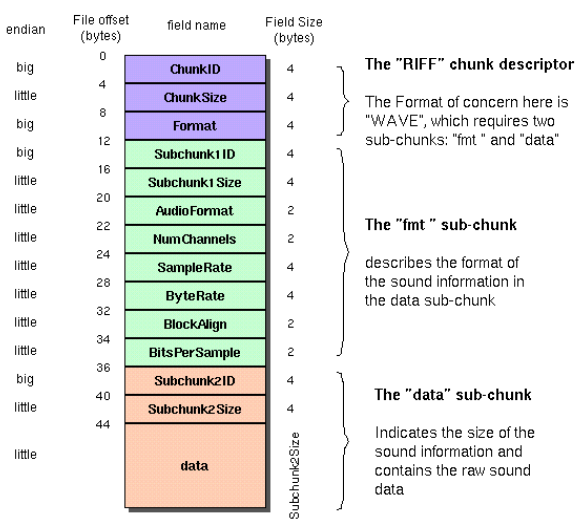
\includegraphics[width=\columnwidth]{images/WaveFormat.png}
\captionof{figure}{The Canonical WAVE file format \cite{website:WAVEFormat}}
\paragraph{{\normalfont After parsing data from the the WAVE file header, we can derive the sample count, audio length, and metadata size by using the following equations:}}

\begin{align*}
&\textit{BytesPerSample} = (BitsPerSample * 8) \\
&\textit{SampleCount} = (Subchunk2Size / BytesPerSample) \\
&\textit{AudioLength} = \\
&{(SampleCount / (SampleRate * NumChannels))} \\
&\textit{MetadataSize} = \\
&{(ChunkSize - (Subchunk1Size + Subchunk2Size)}
\end{align*}

When parsing audio, each sample is defined by a signed number with a bit length as defined in the WAVE header. This number represents a digital measurement from a reference point at 0 dB. For our steganographic methods to be effective, we will need encode our hidden data in a manner that produces a new waveform that is indiscernible from the original.

\noindent
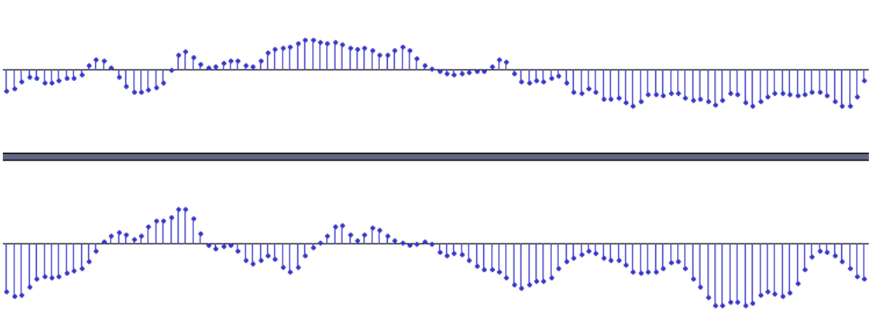
\includegraphics[width=\columnwidth]{images/sample_rate.png}
\captionof{figure}{2 channel 44100 Hz WAVE audio samples}

\section{Steganography}
The motivation behind employing steganographic techniques, as formulated by Djebbar, et al., "is to reliably send hidden information secretly." \cite{paper9} This central need for secrecy promoted the development of a means of encoding data into audio files that hampers detection of the hidden data via LSB statistical analysis. Furthermore, experts only consider audio steganography to be successful if both the modified signal is indistinguishable from the original and embedded messages are fully recoverable \cite{paper3}. Therefore, we must ensure that any processes in our encoding algorithm are both covert and reversible. 

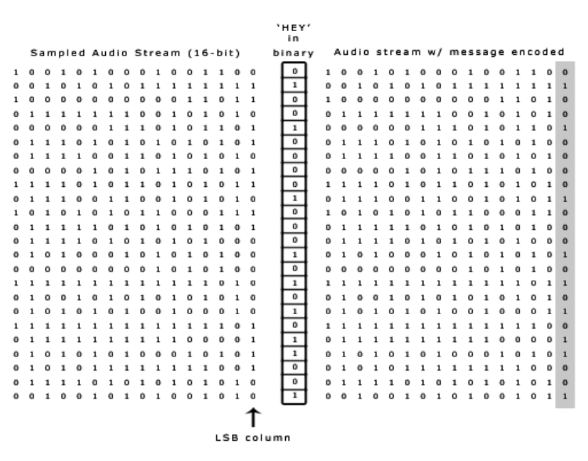
\includegraphics[width=\columnwidth]{images/lsb_example.png}
\captionof{figure}{Example of LSB Steganography in a 16-bit audio stream \cite{paper6}}

The first problem we faced when designing an algorithm for performing LSB Steganography was determining the number of bits to use per sample during encoding. Methods for increasing the capacity of LSB-based audio steganography have been proposed by utilizing three to four least significant bits of an encoding medium \cite{paper4}. We acknowledge that using more than one least significant bit in our audio samples would increase the capacity of data we could store; however, one of the goals of our algorithm is to minimally alter the transmission medium. Therefore, we use only a single LSB per sample to carry our encoded data. The next issue we faced was the determination of how many bits to read during the decoding process. To encode data, we simply convert data into a bitstream and encode it within the LSB column of aligned audio samples. For decoding, we need to know how many bits must be extracted to restore the original data. The first technique we considered was to write a bitstring with padding. The padding would consist of a single 1 bit followed by enough 0 bits to fill the remaining samples. During decoding, we simply identify the point at which this pattern occurs and extract the LSB bits up to that location. There are a few issues with this method. Research has shown that the less information that is embedded into a transmission medium for steganography, the smaller the probability of introducing detectable artifacts during the embedding process \cite{paper1}. If we include a padding, we are potentially modifying the transmission medium more than necessary. Additionally, a series of 0's would likely be noticeable to LSB Steganography detection techniques. The next method we considered was to write the encoded bitstring length in a fixed-size header. To decode, we could read the header value and then read that many bits. One advantage of this solution over the first one is that we avoid writing an unnecessary series of 0's, which could be quite large if the data we encoded is small relative to the sample space. Unfortunately, this technique also has a few disadvantages: we are forcing a maximum encoded file size based on the largest number that can be represented by our fixed-size header, and we are forcing a minimum audio sample count based on that same number, if we are to avoid the potential for data overflow. Our solution was to calculate a variable length header based on the encoding medium size, or the number of samples within an audio file. We simply need enough binary digits to represent the maximum sample count. Headers with a bit length beyond that size unnecessarily alter the encoding medium. We determined that our header bit length should be calculated by $\lceil\log_2(\textit{sample\_count})\rceil$. We can then calculate the header value by multiplying the number of bytes in our encoded data by 8, the number of bits per byte. This technique allows us to encode data within a header size as small as 1 bit. The maximum header size is defined by the number of samples within the audio, achieving a variable length header. To decode, we calculate $\lceil\log_2(\textit{sample\_count})\rceil$ to identify the number of bits associated with our header, read the value of the header, and then read that many bits from the remaining LSB bit-vector. This method addresses all of the disadvantages in the first two propositions. To ensure reliability, we added error checking to JackTheRIFFer to determine when users attempt to encode data that is larger than the available sample space. We must also consider that the encoded data will be encrypted by AES with a 128 bit key. Therefore, the maximum data in bytes that we can store is $\lfloor\frac{sample\_count - header\_bit\_length - key\_size}{8}\rfloor$. The relevant equations for the processes described in this section are provided below:

\begin{align*}
&\textit{header\_bit\_length} = 
\lceil\log_2(\textit{sample\_count})\rceil \\
&\textit{header\_value} = data\_byte\_count \cdot 8 \\
&\textit{key\_size} = 128 \\
&\textit{max\_data\_bytes} = \\
&\lfloor\frac{sample\_count - header\_bit\_length - key\_size}{8}\rfloor \\
\end{align*}

\subsection{Cryptography}
One of our goals is to provide security even when implementation details are known.
By encrypting data before it is encoded, we increase the entropy of data within the LSB bit-vector. This defeats techniques such as sample pair analysis \cite{paper2}, which rely on probabilistically detecting LSB Steganography based on the occurrence of commonly observed consecutive bit patterns. While we believe we are the first to combine cryptography with our previously proposed steganographic algorithm, we acknowledge previous research in applying cryptographic methods to LSB Steganography \cite{paper8}. We decided to use the Advanced Encryption Standard (AES) with a 128-bit key and Cipher Block Chaining (CBC). The key value is determined by a 16-byte ASCII password entered by the user during interaction with the JackTheRIFFer executable. Passwords less than 16-bytes are accepted and padded to the appropriate length. When this occurs, users are notified that their key has been padded and as a result it may be considered less secure. The padding byte we chose is the ordinal value of the ASCII character for the number zero. During encryption, the data to be encrypted is padded to a multiple of 128 bits. This padding is performed by appending the EOF character and the necessary number of additional bytes to reach a multiple of 16. After decryption, the order of the decrypted data is reversed. Then the location of the EOF byte is found, and all bytes up to and including that byte are discarded. The bytestream is again reversed, and the original data is recovered.

\subsection{Encoding}
To initiate the encoding process, a user provides an encryption key, a file to encrypt and encode, an audio file in the WAVE format, and an output filename. The encryption key is padded to 128 bits if necessary, and the input file is encrypted using the Advanced Encryption Standard and Cipher Block Chaining. The encrypted file is then converted into a bitstream. The header size and value are calculated using the techniques described in the Steganography section. Then, the LSB bit-vector of the samples within the WAVE file is steganographically encoded with the header and the encrypted bitstream. This process is illustrated in Figure 4 for reference.            
\vspace{4 mm}

\noindent
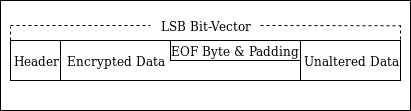
\includegraphics[width=\columnwidth]{images/LSBBitVectorSmall.png}
\captionof{figure}{Diagram of the data encoded within a LSB Bit-Vector}



\subsection{Decoding}
To initiate the decoding process, a user provides a decryption key, a previously encoded audio file in the WAVE format, and an output filename. Keys with a length less than 128 bits are padded accordingly. The header size is calculated using the technique described in the Steganography section. Then, the value of the header is extracted from the LSB bit-vector in the audio samples. A number of bits indicated by the header are read from the remaining audio samples and stored as a large bitstring. This bit string is then converted into an array of bytes and decrypted using the techniques described in the Cryptography section. The result is written to a file.

\section{Evaluation}
We tested JackTheRIFFer by encoding text, audio, video, and executable programs into various WAVE files and we were consistently able to successfully extract the encoded and encrypted data. If invalid decryption keys were provided, the resulting data was garbled and it did not represent the original information that was hidden. We found that audio samples were minimally altered during the encoding process, and modifications to WAVE files were undetectable by listening to the audio. We measured the entropy of WAVE files before and after using LSB Steganography with JackTheRIFFer and found that both observations maintained a similar relative entropy.

\noindent
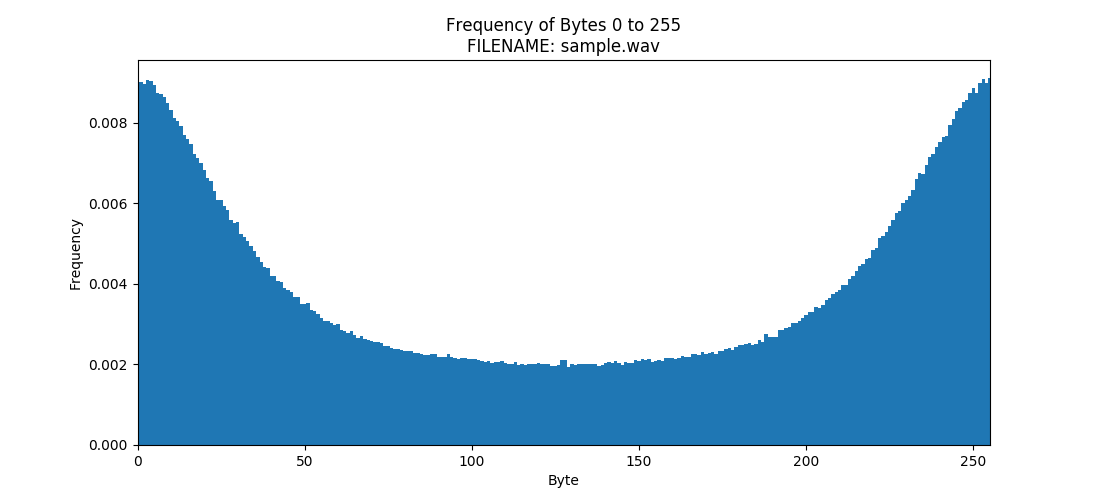
\includegraphics[width=\columnwidth]{images/before.png}
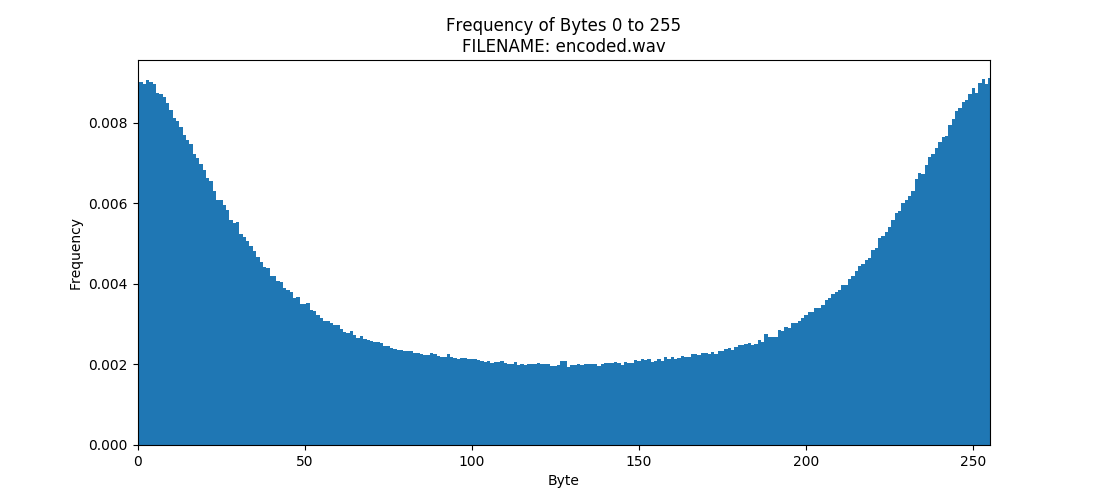
\includegraphics[width=\columnwidth]{images/after.png}
\captionof{figure}{Entropy measurements before (top) and after (bottom) LSB steganography using JackTheRIFFer}

\section{Conclusion And Future Work}
Throughout the development of this utility we identified various enhancements that could be made for future iterations. First, it seems very beneficial to encrypt the JackTheRIFFer header along with the hidden data. This would make it difficult for observers to identify and calculate the header value when analyzing an audio file potentially encoded with JackTheRIFFer. In the current implementation, the encrypted data can be extracted from the LSB bit-vector fairly easily; although, the AES decryption key would still be needed to restore the original data. We also would like to consider adding support for additional audio formats in the future, including AIFF, FLAC, and mp3. Although this work concentrates on audio file formats, similar techniques could be applied to alternative media such as images and video. The security of our implementation could be improved by increasing the AES key-size, as well as loading the key from a file, which could potentially avoid limiting users to entering passwords in the printable character range. Furthermore, the use of public key algorithms instead of AES would offer several benefits, such as stronger key generation and the ability to send messages asymmetrically. The inclusion of a Message Authentication Code (MAC) would be a useful feature to provide for integrity checking. If a user has the original audio file and an encoded file, they could perform steganalysis and determine the range of encoded bits with reasonable accuracy. Adding noise to random LSB bits outside the range of encoded data could address this issue, but we would no longer be minimally altering the transmission medium. We are considering adding an option for this technique so users can utilize it in situations where it may be useful. While the encoding technique presented in this paper is novel, we have found a number of ways in which it could be improved. One issue with the current technique is that we begin encoding on the first audio sample. Instead of starting at LSB\_sample[0] we could potentially hash the key provided by the user and start the encoding sequentially at LSB\_sample[i] where,\\
\textit{i = hash(key) mod n, \\
n = (sample\_count - header\_size - encrypted\_data\_size).}


This technique strengthens support for our goal of providing security even when implementation details are known and also creates additional difficulties for steganalysis. An alternative to encoding data sequentially would be to create a non-repeating sequence of LSB samples to encode. We can use Euler's Theorem to take advantage of the following: \\ \textit{$\alpha ^{\varphi(sample\_count)} \equiv$ 1 (mod sample\_count).}
\vspace{2 mm} \\
Therefore, the user provided key could be used as input to a function that produces a generator $\alpha$ such that $\alpha$ and $\varphi$(\textit{sample\_count}) are coprime. Then, we could encode each i\textsuperscript{th} bit in our encrypted bitstream as: \\
LSBSample[\textit{$\alpha ^{i}$ mod sample\_count}] = \textit{encrypted\_data[i]}.
\vspace{2 mm} \\
Several of these techniques could be used in unison to create a highly versatile steganographic routine. We are also interested in exploring alternative encoding techniques such as wavelet domain LSB insertion as proposed by other experts \cite{paper7}. In conclusion, we identified a variety of methodologies in which LSB steganography can be applied to audio file formats such as WAVE, designed a novel technique for performing covert and reliable steganography with AES encryption, and implemented the algorithms we designed into a functional prototype.
